\documentclass[11pt]{article}

\usepackage[margin=1in]{geometry}
\usepackage{amsmath, amssymb}
\usepackage{graphicx}
\usepackage{enumitem}
\usepackage{fancyhdr}
\usepackage{hyperref}
\usepackage{minted}

\pagestyle{fancy}
\fancyhf{}
\lhead{ENPM701 --- Homework 4}
\rhead{Marcus Hurt}
\cfoot{\thepage}

\title{Homework 4}
\author{Marcus Hurt \\ \href{mailto:mhurt@umd.edu}{mhurt@umd.edu}}
\date{ENPM701: Autonomous Robotics}

\begin{document}

\begin{titlepage}
    \centering
    \vspace*{2in}
    {\LARGE\bfseries Homework 4\par}
    \vspace{0.5in}
    {\Large ENPM701: Autonomous Robotics\par}
    \vspace{1in}
    {\large Marcus Hurt\par}
    \href{mailto:mhurt@umd.edu}{mhurt@umd.edu}
    \vfill
    {\large University of Maryland\par}
    {\large \today\par}
\end{titlepage}

\section*{Question \#1 (10 points)}

The object and the measured distance to it can be seen below.

\begin{figure}[h]
    \centering
    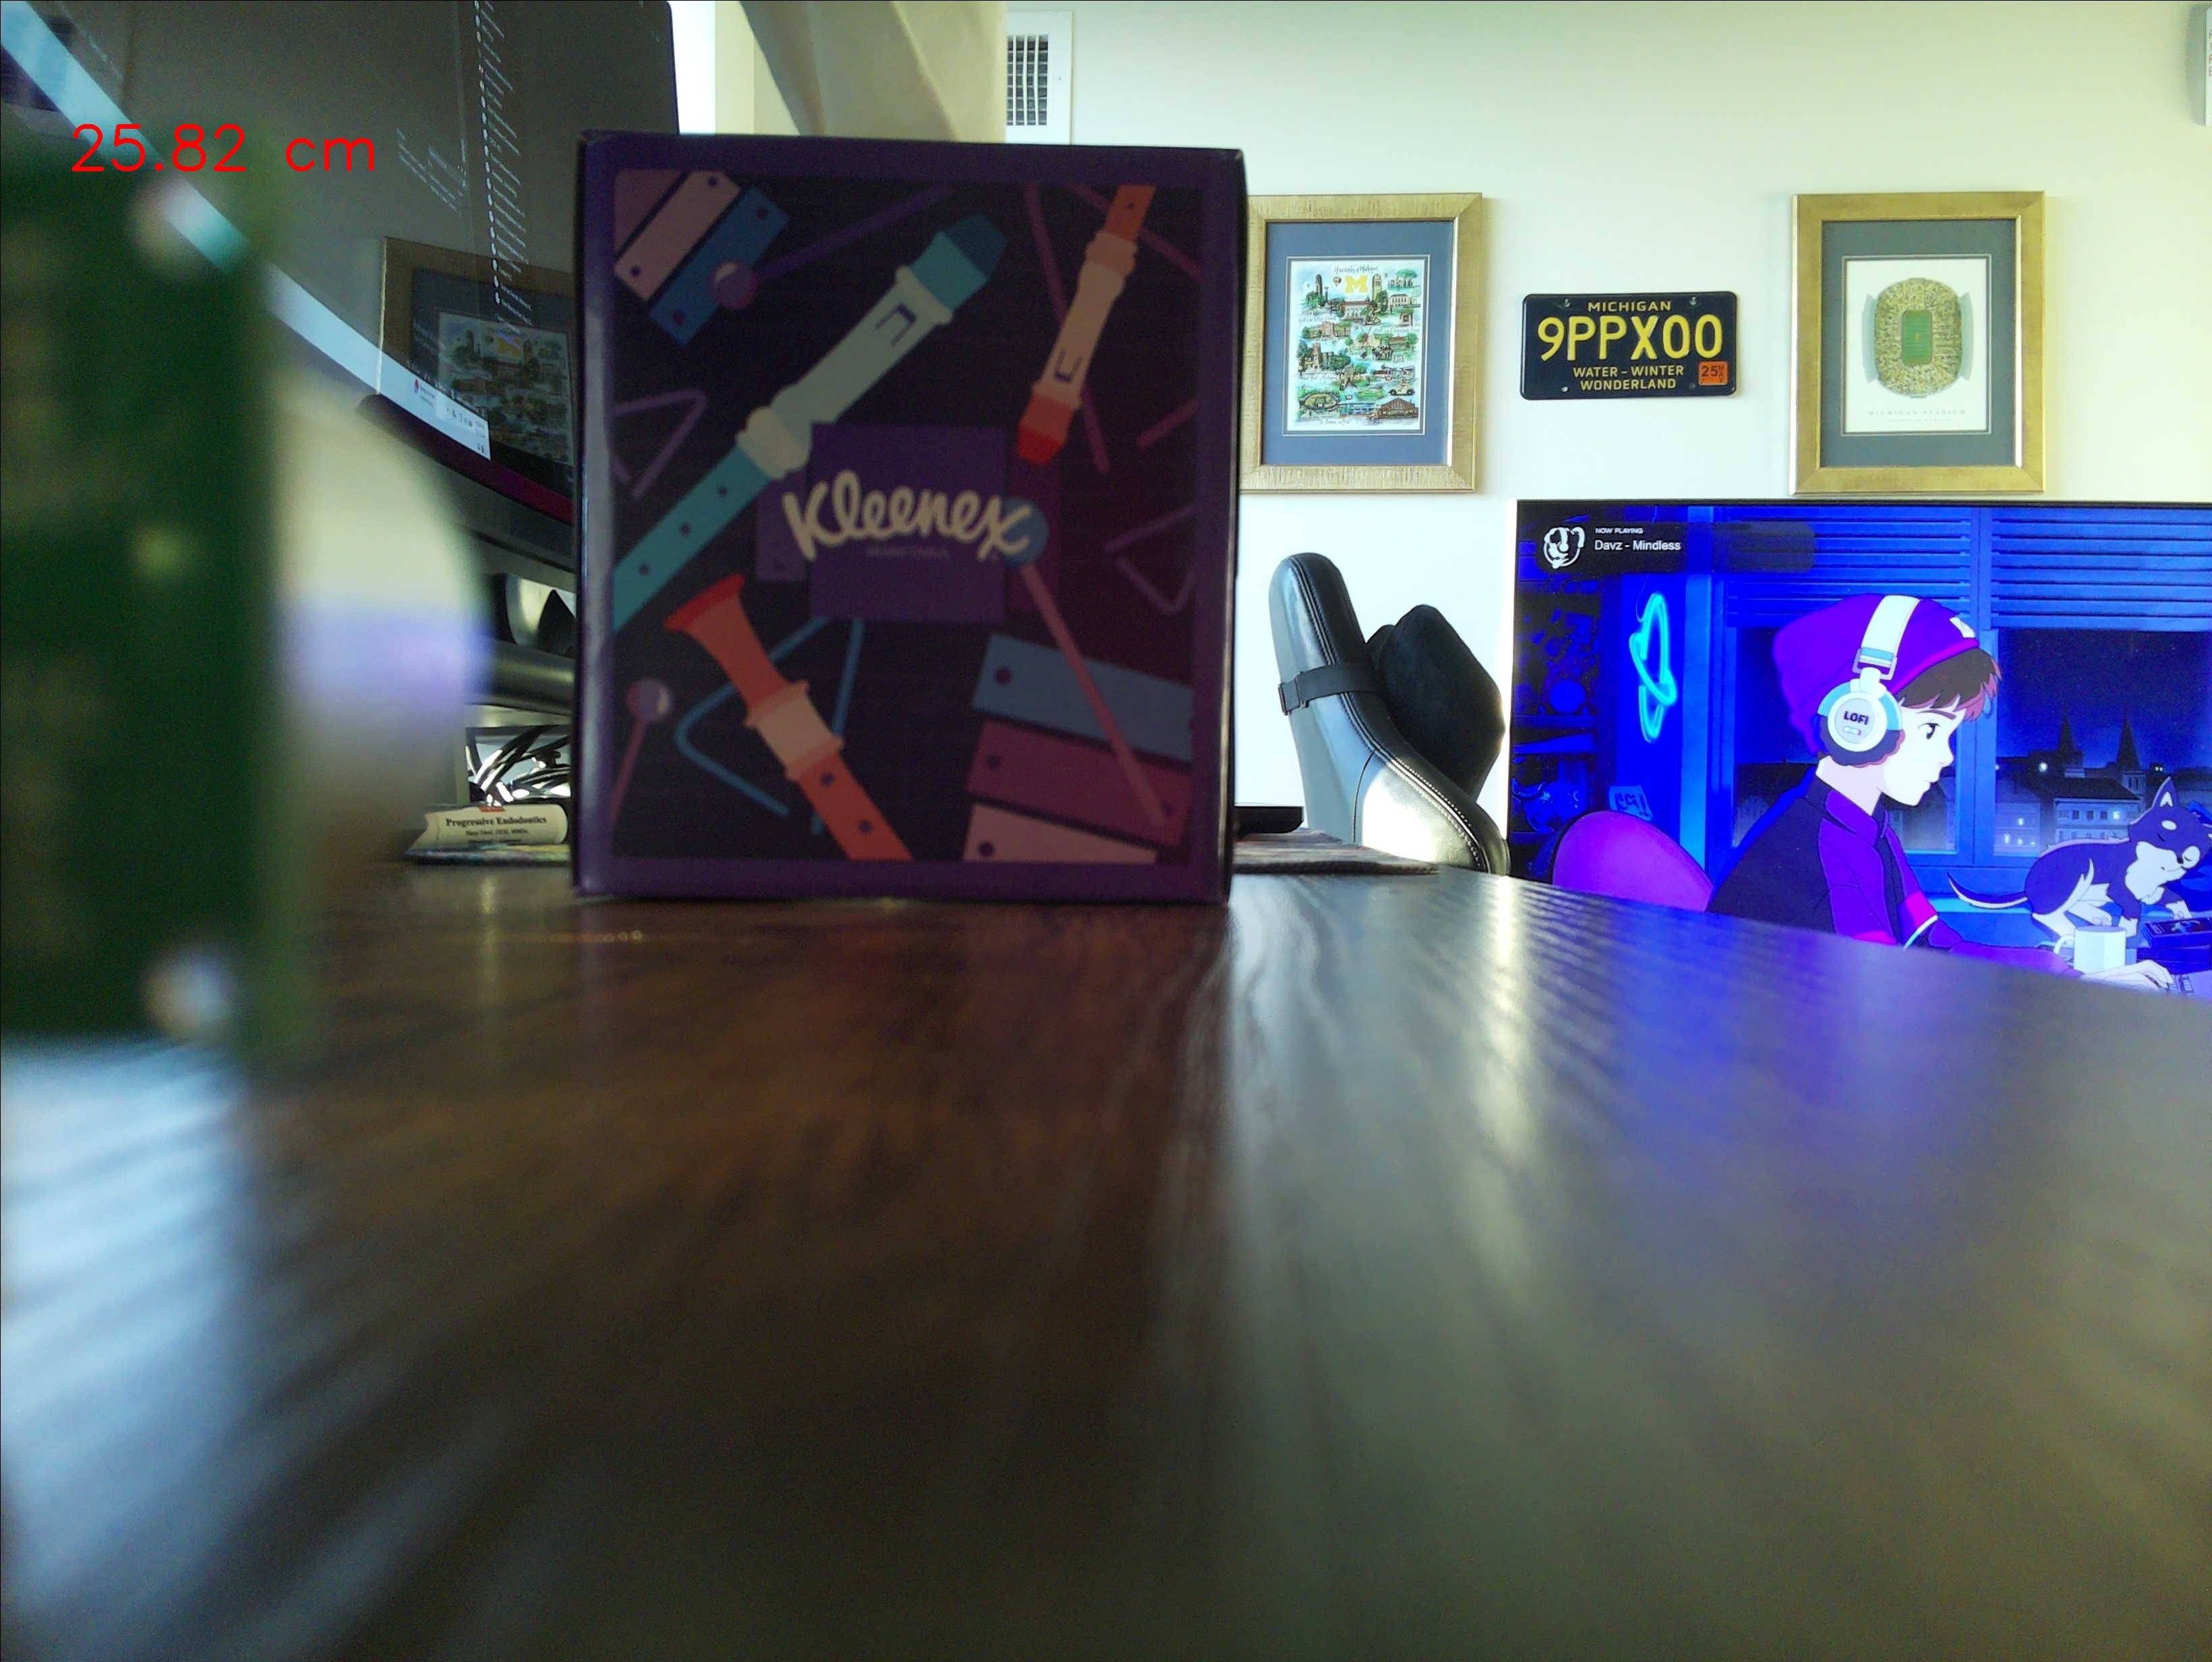
\includegraphics[width=0.8\textwidth]{DistanceMeasurement.jpg}
    \caption{Data Visualization of Green Light Detection}
    \label{fig:distance_measurement}
\end{figure}

\section*{Question \#2 (10 points)}

\subsection*{Step 7}

View the video below. It shows the arrrow detection in action.

\url{https://youtu.be/yPdmxDvLtlw}

\subsection*{Step 8}

This analysis was very intereseting. The video frame rate had to be reduced to 10 frames per second in order to be able to process the frames in real time. The detection was mostly accurate. This highlights the limitations of the Pi processor. We could only process frames in around 60 ms with some even taking longer, which is not ideal for real-time applications. This could be improved by using a more powerful processor or optimizing the code further.

\begin{figure}[h]
    \centering
    
\includegraphics[width=0.8\textwidth]{frame_times.png}
    \caption{Data Visualization of Arrow Detection}
    \label{fig:data_visualization_arrow_detection}
\end{figure}

\end{document}
